\chapter{Background}\label{cha:chapter3}

\section{Neural Networks}
Neural networks(NNs) are a type of machine learning algorithms that inspired by how human brain works.  In particular, NNs have units called neurons connecting together similar to the way of neurons our brain do. These connections allow NNs to hierarchically build representations that are necessary to perform an objective task. \addfigure{\ref{fig:nn_simple}} illustrates a simple coordination reaction task by our brain.

 \begin{figure}[ht!]
    \begin{center}

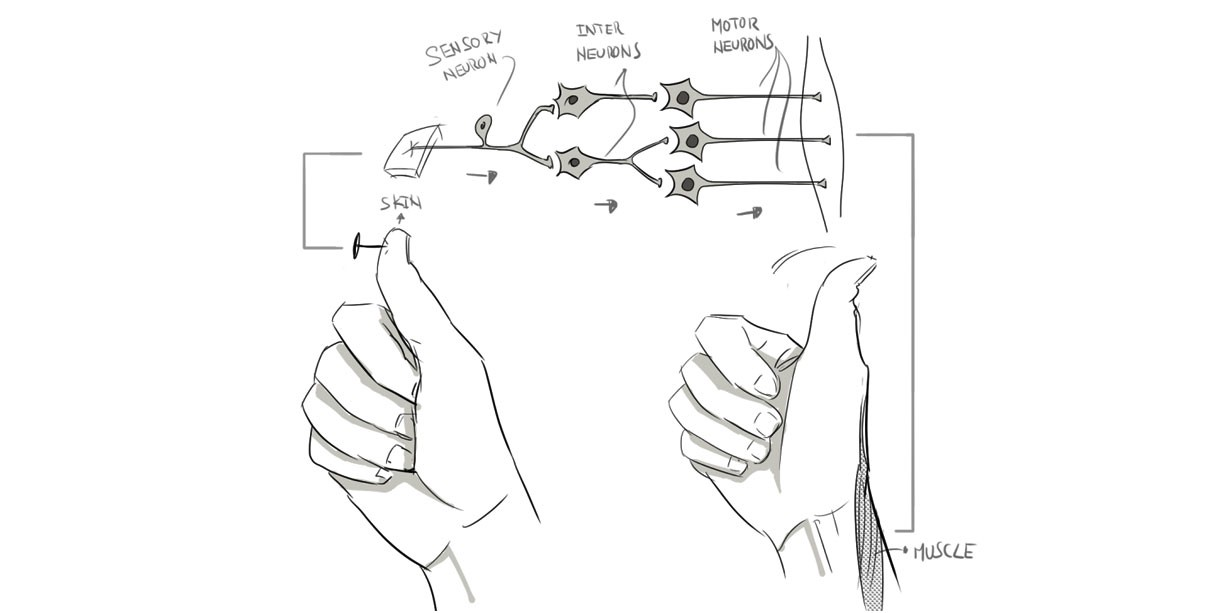
\includegraphics[width=\textwidth]{nn_simple}
\caption[xxx]{An illustration of how neurons in human brain cooperate together to sense the pain and react accordingly. \footnotemark}
\label{fig:nn_simple}

\end{center}
\end{figure}
\footnotetext{Source: Eugenio N. Leon, \url{https://becominghuman.ai/making-a-simple-neural-network-2ea1de81ec20}}


 \begin{figure}[ht!]
    \begin{center}

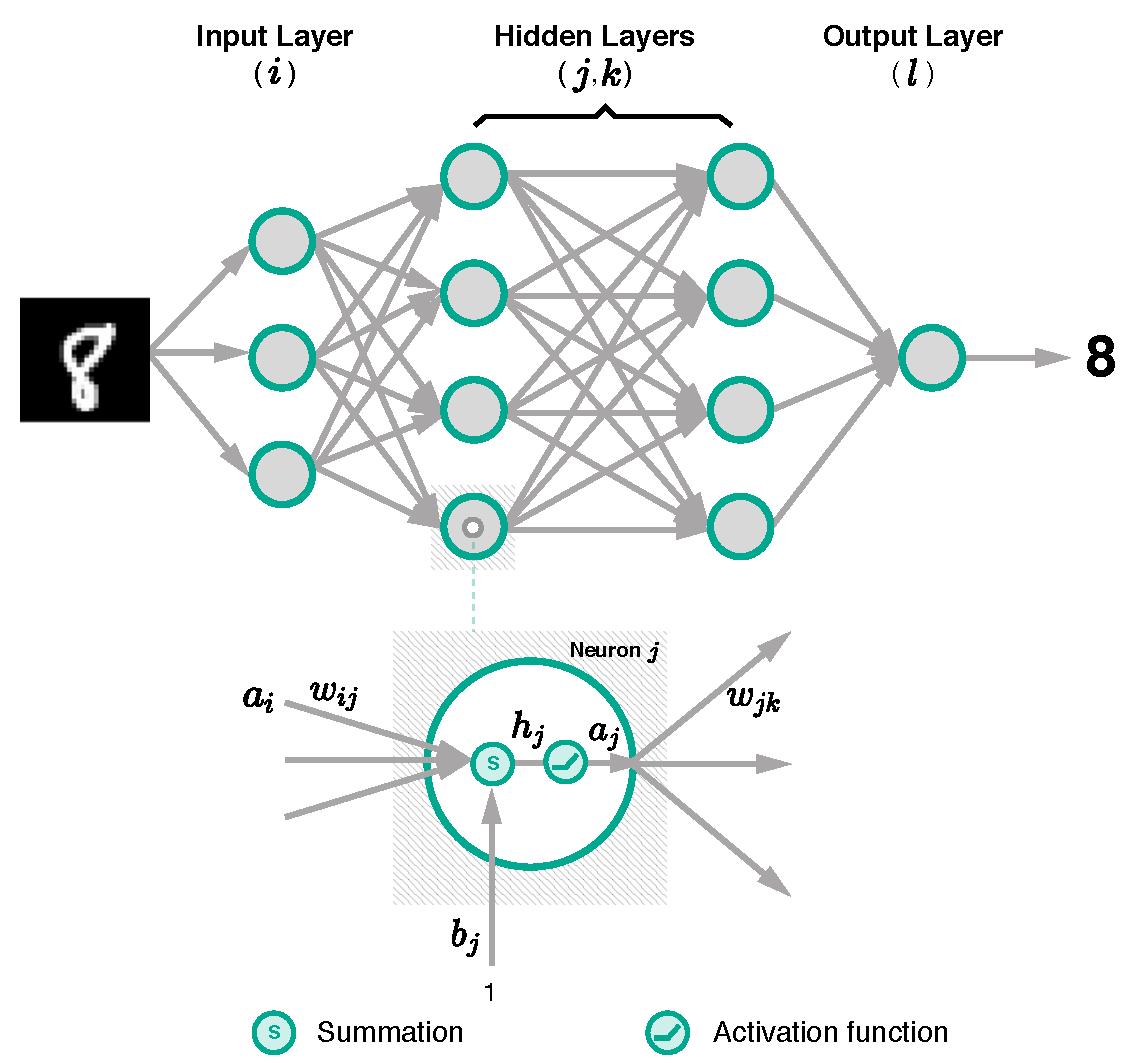
\includegraphics[width=0.8\textwidth]{sketch/typical_nn_structure}
\caption[]{A general structure of neural networks}
\label{fig:nn_typical_structure}

\end{center}
\end{figure}


 \begin{figure}[ht!]
	\begin{center}

		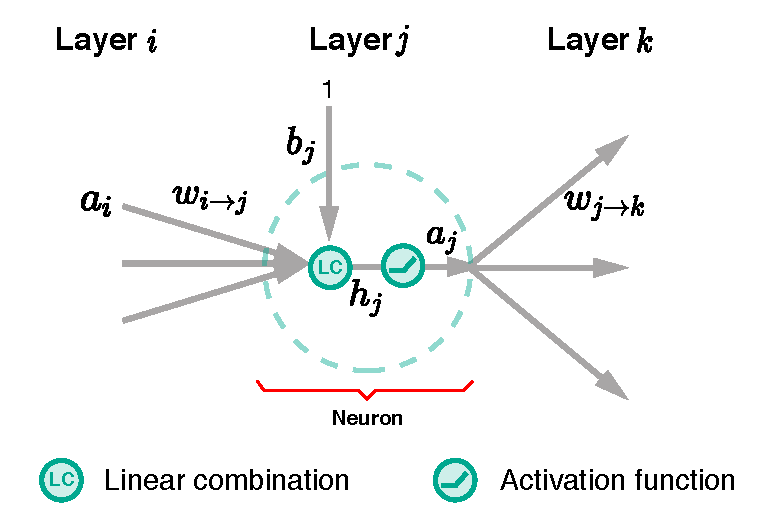
\includegraphics[width=0.5\textwidth]{sketch/a_neuron}
		\caption{Connectivity of a neuron}
		\label{fig:a_neuron}
	\end{center}
\end{figure}


\addfigure{\ref{fig:nn_typical_structure}} illustrates a general structure of NNs. It has input layer, output layer and hidden layers, which are analogously similar to sensory, motor and inter neurons in \addfigure{\ref{fig:nn_simple}}. \addfigure{\ref{fig:a_neuron}} shows connections of a neuron to neurons in previous and later layer. The goal is to build connections between these neurons such that the NN is able to perform an objective task with high accuracy.  These connections are determined by weights, which are denoted by $w_{i\rightarrow j}, w_{j\rightarrow k}$ in \addfigure{\ref{fig:a_neuron}}. This process is called \textit{training}.  In this example, the objective task to classify what is the given digit.


Consider a given set of $p$ training samples $\mathcal{D} = \{ \xa, \ya) \}_{\alpha=1}^{p}$,  there are 3 primary components to train a NN, namely  
\begin{enumerate}
	\item \textbf{Network architecture} : $\sigma$ it defines how neurons connect and communicate to each other. More precisely, these are corresponding to connection weights and biases $\patvector{\theta}$ and neuron's activation functions illustrated in \addfigure{\ref{fig:nn_typical_structure}}. Mathematically, it is a function $f$ with parameters $\patvector{\theta}$ that nonlinearly transforms an input $\xa\in \mathbb{R}^d $ to some values.
	\item \textbf{Loss function $L$} : it is a measurement corresponding to the objective task that quantifies whether output $f(\xa)$ from the NN matches the true output $\ya$.
	\item \textbf{Learning algorithm} : it is responsible to find the network's parameters $\patvector{\hat{\theta}}$ to optimize the loss function $L$(\textit{Empirical Error})  as a proxy for optimizing loss or error for unforeseen $\x \notin \mathcal{D} $ (\textit{Generalization Error}). 
\end{enumerate}

Hence, the goal of this empirical training process can be summarized as follows : 

\begin{align}
	\patvector{\hat{\theta}} = \patarg{min}{\theta} \sum_{\alpha=1}^p L( f(\xa), \ya) 
\end{align}

\subsection{Loss functions}
Choosing loss function is depend on the objective of problem that the NN is being trianed to to solve. For classification problems, such as digit classification, which the goal is to categorize $\x$ into $K$ categories $C$, $f : \x \in \mathbb{R}^d  \mapsto C \in \{ C_k \}$, \textit{Cross-Entropy}(CE) is the loss function for this purpose.
$$
l_{\text{CE}} = - \sum_{i} y_k \log \hat{y}_k,
$$
where $y_i \in [0, 1]$ and $\hat{y}_i \in [0, 1]$ are true and predicted probability that $\x$ belongs to $C_k$ respectively. Consider a $K$-class classification problem, $\patvector{z} = f(\x) \in \mathbb{R}^{K}$, $\hat{y}_k$ is computed via \textit{softmax} activation function :
$$
\hat{y}_k = \frac{e^{z_k}}{ \sum_{k=1}^K{e^{z_k}} }
$$ 

For regression problems, $ f : \x \in \mathbb{R}^d  \mapsto \mathbb{R}$, such as forecasting price, requires \textit{Mean Squared Error}(MSE) loss function.
$$
l_{\text{MSE}} = (f(\x) - y)^2
$$

This is a brief introduction to loss functions widely used in machine learning. More loss functions do exist and are beyond scope of the thesis to cover.

\subsection{Learning Algorithm : Gradient Descent and Backpropagation}
Consider a  function $L(\theta) = \theta^2$ on \addfigure{\ref{fig:gradent_descent_toy}} as a simplified version of loss function averaged over all $\xa \in \mathcal{D}$  from a NN with a parameter $\theta$. In this case, $\hat{\theta}$ can trivially computed by solving

\begin{align}
	\frac{d L(\theta)}{d \theta}  \stackrel{!}{=} 0
	\label{eq:simple_solve_for_thetha}
\end{align}

\begin{figure}[ht!]
    \begin{center}
		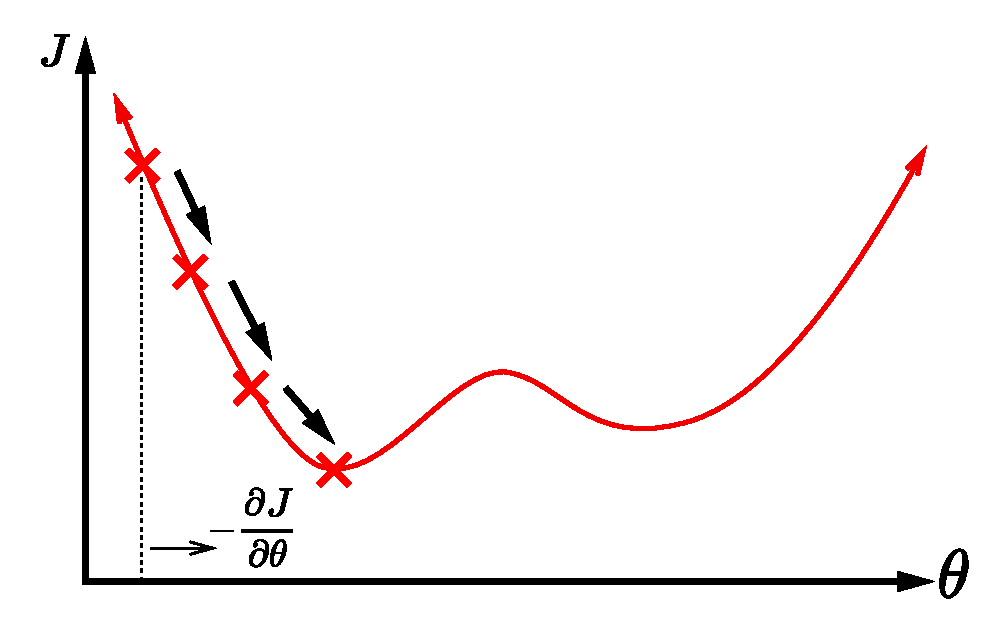
\includegraphics[width=0.6\textwidth]{sketch/gradient_intuition}
		\caption[]{An illustration of Gradient Descent}
		\label{fig:gradent_descent_toy}
	\end{center}
\end{figure}

However, a NN usually contains thousands of parameters, hence $L(\boldsymbol{\theta})$ becomes a high dimensional function and solving ($\ref{eq:simple_solve_for_thetha}$) is not a trivial task. Nonetheless, \addfigure{\ref{fig:gradent_descent_toy}} shows an insight how we can reach the minimum location. There, we can see that if we move $\theta$ in the opposite direction of gradient $	-\frac{d L(\theta)}{d \theta}$ with a proper step size $\lambda$ (\textit{learning rate}), we will eventually reach the minimum. Therefore, instead of directly solve ($\ref{eq:simple_solve_for_thetha})$, we rather slightly adjust $\btheta$ in the same direction of the gradient for some iterations, for example until the loss function converges. This is called \textit{Gradient Descent}.

\begin{align*}
\forall \theta_i \in \btheta :  \theta_i \leftarrow \theta_i - \frac{\lambda}{p} \sum_{\alpha=1}^{p} \frac{\partial l(f(\xa), \ya }{\partial \theta_i } 
\label{eq:gradient_update}
\end{align*}


Let's consider again a simple NN shown in \addfigure{\ref{fig:nn_typical_structure}} with $\btheta = \{ \forall i,j,k,l : w^{(1)}_{i \rightarrow j}, w^{(2)}_{j \rightarrow k}, w^{(3)}_{k \rightarrow l}  \}$ and biases are omitted. Then, $f(\x, \btheta)$ is calculated as follows

\begin{align*}
		h_j^{(1)} &= \sum_i w_{i \rightarrow j}^{(1)} x_i & a_j^{(1)} &= \sigma (h_j^{(1)})	\\
		h_k^{(2)} &= \sum_j w_{j \rightarrow k}^{(2)} a_j^{(1)}  & a_k^{(2)} &= \sigma (h_k^{(2)})	 \\
		h_l^{(3)} &= \sum_k w_{k \rightarrow l}^{(3)} a_k^{(2)} & a_l^{(3)} &= \sigma (h_l^{(3)})	 \\
		f(\x) &= [ a_1^{(3)}, \dots, a_L^{(3)}  ]^T  & L &= \frac{1}{p} \sum_{\alpha = 1}^{p} l(f(\xa), \ya)	
\end{align*}

Consider a sample $(\xa, ya)$. The gradients can be computed by recursively applying chain rule to $l$ from the last to the first layer, hence the name \textit{Backpropagation}.
\begin{align}
	\frac{\partial l(f(\xa), \ya)  }{\partial w_{k \rightarrow l}^{(3)} } &= 	\frac{\partial l(f(\xa), \ya) }{\partial a_{l}^{(3)} }  \frac{\partial a_{l}^{(3)} }{\partial w_{k \rightarrow l}^{(3)} }  	\\
		&= 	\underbrace{\frac{\partial l(f(\xa), \ya) }{\partial a_{l}^{(3)} } \sigma'(h_l^{(3)})}_{ \delta_l^{(3)}} a_{k}^{(2)} 	\\
	\frac{\partial l(f(\xa), \ya)  }{\partial w_{j \rightarrow k}^{(2)} } 
		&=  \sum_{l' = 1}^{L} 	\frac{\partial l(f(\xa), \ya) }{\partial a_{l'}^{(3)} } \frac{\partial a_{l'}^{(3)}}{\partial w_{j \rightarrow k}^{(2)}} \\
		&= \sum_{l' = 1}^{L} 	\frac{\partial l(f(\xa), \ya) }{\partial a_{l'}^{(3)} } \sigma'(h_{l'}^{(3)})  \frac{\partial h_{l'}^{(3)} }{\partial w_{j \rightarrow k}^{(2)}} \\
		&= \sum_{l' = 1}^{L} 	\delta_{l'}^{(3)}  w_{k \rightarrow l'}^{(3)} \frac{\partial a_{k}^{(2)} }{\partial w_{j \rightarrow k}^{(2)}} \\
		&= a_{j}^{(1)}  \underbrace{\sigma'(h_{k}^{(2)}) \sum_{l' = 1}^{L} 	\delta_{l'}^{(3)} w_{k \rightarrow l'}^{(3)}}_{\delta_{k}^{(2)}}  \\
	\frac{\partial l(f(\xa), \ya)  }{\partial w_{i \rightarrow j}^{(1)} } &=  x_i  \sigma'(h_{j}^{(1)}) \sum_{k' = 1}^{K} 	\delta_{k'}^{(2)} w_{j \rightarrow k'}^{(2)} 
\end{align}
As shown in the derivation, \textit{Backpropagation} allows us to efficiently compute the gradients by reusing calculated quantities from computation of later layer, for example $\delta_l^{(3)}, 	\delta_{k}^{(2)}$. Moreover, $\delta_l^{(3)}, 	\delta_{k}^{(2)}$ can interpreted as error of the neuron. 

In practice, because the training set usually contains several thousand samples, the gradient update in  (\ref{eq:gradient_update}) would require significant amount of computation to update one step, not to mention that it could also result in small gradient update step leading to slow convergence to desire objective performance. Therefore, the training data $D$ is usually divided into batches  $\widetilde{D}_i$  with equal size and perform the gradient update for every $\widetilde{D}_i$. For example, the size of $\widetilde{D}_i$ is usually chosen between 32 and 512 samples. This refers to \textit{Mini-Batch Gradient Descent}.

Lastly, because noise in the data and potentially highly non-smooth of the loss function, learning rate $\lambda$ is a great influential to the training process. More precisely, it should not be too small or too large. This requires some effort and experience in order to get the value right. Some work have proposed alternative update rules aiming to make the training process more stable. For example,  Adaptive Moment Estimation(Adam)\cite{KingmaAdamMethodStochastic2014}  uses adaptive learning rate  and incorporates accumulated direction and speed of the previous gradients (momentum) into the update, hence more consistent gradient and fast convergence. Other similar proposals are RMSProp \cite{TielemanLectureRmsPropDivide2012} and Adadelta \cite{ZeilerADADELTAAdaptiveLearning2012}.


\subsection{Convolutional Neural Networks} \label{sec:conv}
Convolutional Neural Networks(CNNs) refer to neural networks that employ convolutional operators to process information in early layers instead of fully-connected layers(weighted sum). Typically, a convolutional operator is followed by a pooling operator. Using this convolutional and pooling operators allows the NN to extract hierarchical features that are spatially invariant \cite{ZeilerVisualizingUnderstandingConvolutional2013}, hence having higher predictive capability of the NN comparing to traditional fully-connected layers with the same number of parameters.

\afterpage{
\begin{figure}[ht!]
    \begin{center}
		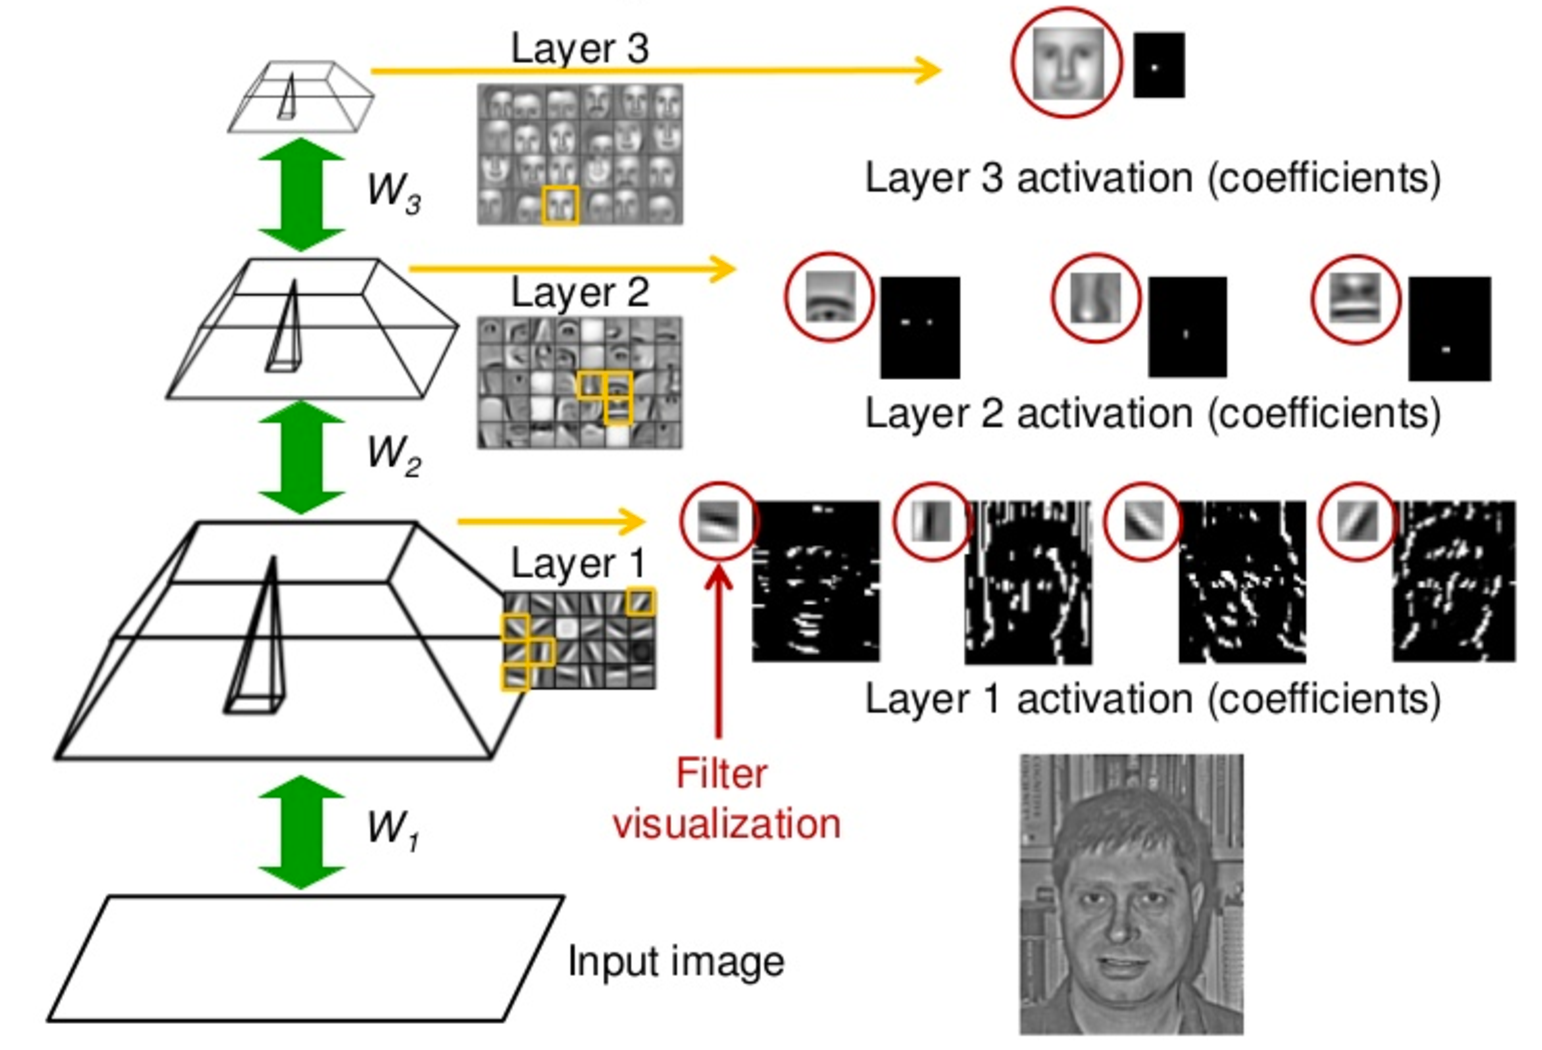
\includegraphics[width=0.5\textwidth]{sketch/cnn_hierachical_features}
		\caption[]{Hierarchical features learned by CNN\footnotemark}
		\label{fig:conv_intuition}
	\end{center}
\end{figure}
\footnotetext{Source : \cite{LeeConvolutionalDeepBelief2009}}
}

\addfigure{\ref{fig:conv_intuition}} illustrates hierarchical structures that CNN's neurons learn to detect. More precisely, in this example, neurons in the first learn to detect low level features, such as edges, and neurons in middle layer then use knowledge to detect higher level features, for example nose, mouth or eyes, and so on.

\afterpage{
\begin{figure}[ht!]
    \begin{center}
		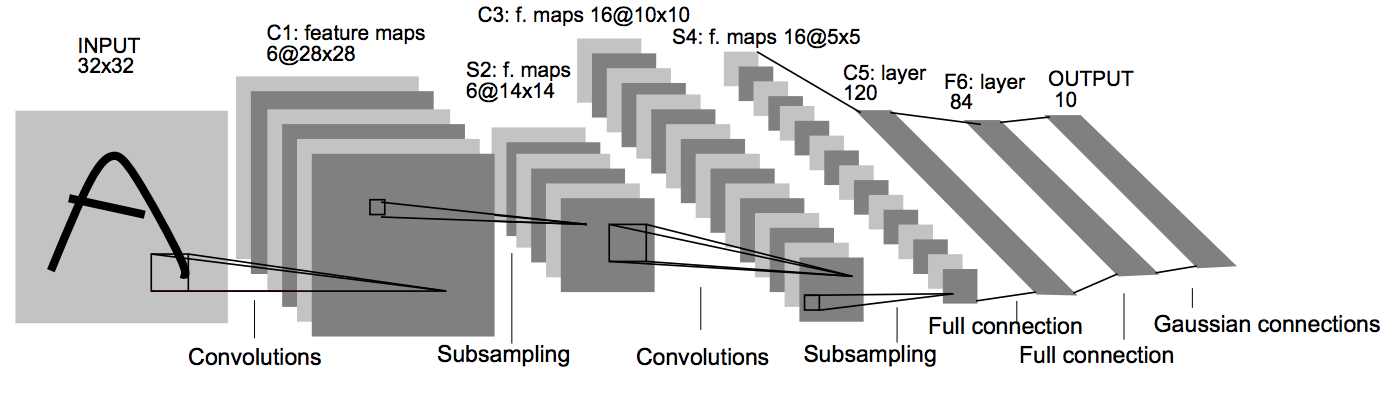
\includegraphics[width=0.8\textwidth]{lenet}
		\caption[xx]{Architecture of LeNet-5 for digits recognition.\footnotemark}
		\label{fig:lenet}
	\end{center}
\end{figure}
\footnotetext{Source : \cite{LeCunGradientBasedLearningApplied2001} }
}

Since \cite{LeCunGradientBasedLearningApplied2001} proposed LeNet-5, shown in \addfigure{\ref{fig:lenet}}, and successfully applied it to handwritten recognition problem, CNNs have become the first choice of architectures in many domains. Particularly, in computer vision, CNNs are the core component of state-of-the-art results in various contests. Such successful results are :  AlexNet\cite{KrizhevskyImageNetClassificationDeep2012} that archive the remarkable results on  ImageNet Large-Scale Visual Recognition Challenge 2012(ILSVRC 2012) followed by the achievement of VGG\cite{SimonyanVeryDeepConvolutional2014} and GoogleLenet \cite{SzegedyGoingDeeperConvolutions2014} architecture in ILSVRC 2014 and ResNet\cite{HeDeepResidualLearning2015} that won ILSVRC 2015.



\subsection{Recurrent Neural Networks}
Recurrent Neural Networks(RNNs) are neural networks whose computed outputs   are repeatedly incorporated into the next computation. \addfigure{\ref{fig:rnn_unfold}} illustrates this idea of recurrent computation by unfolding RNN into steps. Let's consider $\x$ a sequence of $x_1, \dots x_t$.  At step $t$, RNN takes $r_{t-1}$ and $x_{t}$ to compute $r_{t}$ and $\hat{y}_t$. This recurrent connections can be interpreted as accumulating information from the past, hence RNNs are capable of processing sequential data, possibly  coming with different length. Natural Language Processing(NLP) and Machine Translation(MT) are some of the fields that RNNs are widely applied to.

\afterpage{
\begin{figure}[h]
\centering
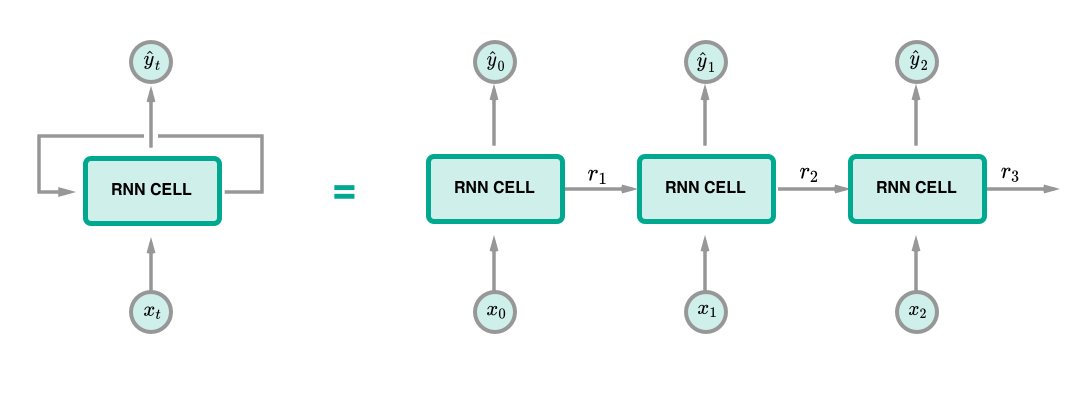
\includegraphics[width=0.8\textwidth]{sketch/rnn_unfold}
\caption[xxx]{Unfolded RNN Structure\footnotemark}
\label{fig:rnn_unfold} 
\end{figure}
\footnotetext{Inspired by \url{http://colah.github.io/posts/2015-08-Understanding-LSTMs/}}
}

\subsubsection{Backpropagation Through Time}
As the number of computation steps in RNNs is depend on the length of samples, which can be different in principle, one needs to organize data in such a way that samples in the same batch have the same steps of computations before training a RNN. In this case, training RNNs can be viewed as training a feedforward neural network where we apply backpropagation,  except that variables are shared across steps. 

Consider again the RNN in \addfigure{\ref{fig:rnn_unfold}} with $\x = \{x_1, \dots, x_T \}$ and $r_0 = 0$. Assume that only $\hat{y}_T$ determines the value of the loss function and the computations are defined as follows 
\begin{align}
	h_1 &= w_{rx} x_1 + w_{rr} r_0 & r_1 &= \sigma(h_1) \label{eq:naive_r} \\
	h_2 &= w_{rx} x_2 + w_{rr} r_1 &  r_2 &= \sigma(h_2) \\
	& \vdots & \vdots \\
	h_{T-1} &= w_{rx} x_{T-1} + w_{rr} r_{T-2} &  r_{T-1} &= \sigma(h_{T-1}) \\
	\hat{y} &= \sigma(w_{yx} x_T   + w_{yr} r_{T-1})
\end{align}

The gradients can be computed by 
\begin{align}
	\frac{\partial l}{\partial w_{yx}} &= \sigma'(w_{yx} x_T   + w_{yr} r_{T-1}) x_T \\
	\frac{\partial l}{\partial w_{yr}} &= \sigma'(w_{yx} x_T   + w_{yr} r_{T-1}) r_{T-1} \\
	\frac{\partial l}{\partial w_{rx}} &= 	w_{yr} \sigma'(w_{yx} x_T   + w_{yr} r_{T-1}) \frac{\partial r_{T-1}}{\partial w_{rx}} \\
	&= w_{yr} \sigma'(w_{yx} x_T   + w_{yr} r_{T-1})  \Bigg[ \sigma'(h_{T-1}) \bigg( x_{T-1} + w_{rr}  \frac{\partial r_{T-2}}{\partial w_{rx}} \bigg) \Bigg]  \label{eq:gradient_wrr}  \\
	\frac{\partial l}{\partial w_{rr}} &= w_{yr} \sigma'(w_{yx} x_T   + w_{yr} r_{T-1})  \frac{\partial r_{T-1}}{\partial w_{rr}}  \\
	&= w_{yr} \sigma'(w_{yx} x_T   + w_{yr} r_{T-1})  \Bigg[ \sigma'(h_{T-1}) \bigg( \frac{\partial r_{T-2}}{\partial w_{rr}} \bigg) \Bigg] \\
\end{align}
However, as we unfold the computations, we can see that there are 2 possibilities that might happen to the gradients of the shared parameters $w_{rx}$ and $ w_{rr}$, namely
\begin{itemize}
	\item Exploding Gradient : this scenario happens if the gradient is derived from shared weights, for example $w_{rr}$ in  (\ref{eq:gradient_wrr}), whose absolute value is greater than one. The recursive multiplication will result in a large value of the gradient leading to unreliable training. \cite{PascanuUnderstandingexplodinggradient2012} have proposed Gradient Clipping to alleviate the problem.
	\item Varnishing Gradient : in contrast, when the values are smaller than one, the gradient will be very small causing slow learning. More precisely, RNNs would require enormous of time to learn long term dependencies. The next section discusses techniques to mitigate this problem
\end{itemize}


\subsubsection{Long Short-Term Memory and Gated RNNs}
Varnishing Gradient is a major problem that causes RNNs to learn long term memories with slow progress. This is due to how the computation of recurrent connections are constructed. In particular, as in (\ref{eq:naive_r}), standard RNNs compute those connections with weighted sum at every step $t$ leading to recursive multiplication terms in the gradient's computation.

Alternatively,\cite{HochreiterLongshorttermmemory1997} have proposed \textit{Long Short-Term Memory}(LSTM) network that employs a gating mechanism and additive updates in the calculation of the recurrent connections. This mechanism decreases number of damping factors involved in the gradients' computation, hence it allows the network to learn long memories better.

More precisely, as shown in \addfigure{\ref{fig:lstm_structure}}, LSTM utilizes 3 gates, namely input $i_g$, forget $f_g$ and $o_g$ output gate, to control the information flow through the LSTM cell. In particular, $i_g$ and $f_g$ decides how to accumulate information in the cell state $C_t$ from previous cell state $C_{t-1}$, previous output $h_{t-1}$ and current input $x_t$, while $o_g$ determines to the information in $C_t$ leaks to outside $h_t$. Formally, 
\begin{align}
	i_g &= \sigma( w_{ix} x_t + w_{ih} h_{t-1} )  &  	f_g &= \sigma( w_{fx} x_t + w_{fh} h_{t-1} )\\
	o_g &= \sigma( w_{ox} x_t + w_{oh} h_{t-1} ) & \widetilde{C}_t &= \tanh(w_{cx} x_t + w_{ch} h_t) \\
	C_t &= f_g \odot C_{t-1} + i_g \odot \widetilde{C}_t & h_{t} &= o_g \odot\tanh(C_t)
\end{align}


\begin{figure}[h]
\centering
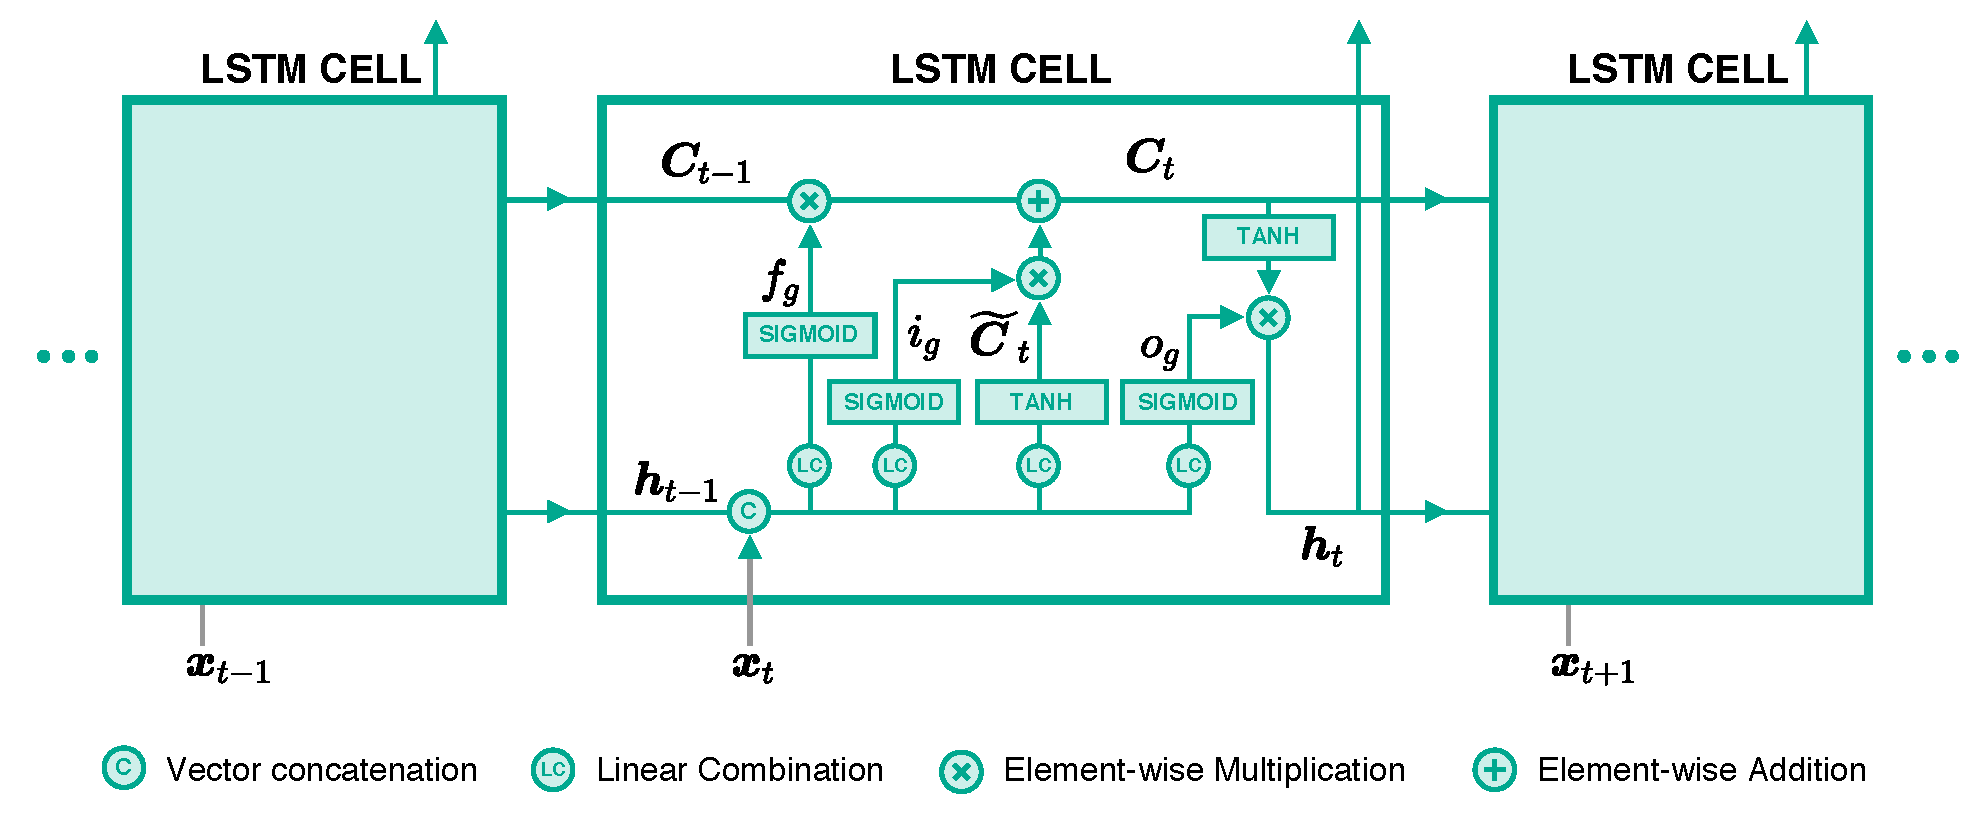
\includegraphics[width=1\textwidth]{sketch/lstm}
\caption{LSTM Structure} 

\label{fig:lstm_structure} 
\end{figure}

Since the work published, LSTM has successfully contributed to many state-of-the-art results, such as MT ..... \cite{GreffLSTMsearchspace2017} have shown that the forget and output gate are the crucial parts of the network.  \cite{ChoLearningPhraseRepresentations2014a} have proposed \textit{Gated Recurrent Unit}(GRU) that employs only 2 gates, however \cite{Jozefowiczempiricalexplorationrecurrent2015a} have conducted several benchmarking tasks and found no significant difference in performance between LSTM and GRU. 